%----------------------------------------------------------------------------------------
%	PACKAGES AND OTHER DOCUMENT CONFIGURATIONS
%----------------------------------------------------------------------------------------

\documentclass[11pt,a4paper]{article}

\usepackage[utf8]{inputenc}
\usepackage[dutch]{babel}
\usepackage{amsmath}
\usepackage{amsfonts}
\usepackage{amssymb}
\usepackage[left=2cm,right=2cm,top=2cm,bottom=2cm]{geometry}
\usepackage{graphicx}
\usepackage{float}
\graphicspath{{figures/}}
\usepackage{todonotes}

%----------------------------------------------------------------------------------------
%	CONFIGURATION OF CODE LISTINGS
%----------------------------------------------------------------------------------------

\usepackage{listings}
\usepackage{color}
 
\definecolor{codegreen}{rgb}{0,0.6,0}
\definecolor{codegray}{rgb}{0.5,0.5,0.5}
\definecolor{codepurple}{rgb}{0.58,0,0.82}
\definecolor{backcolour}{rgb}{0.95,0.95,0.92}
 
\lstdefinestyle{mystyle}{
    backgroundcolor=\color{backcolour},   
    commentstyle=\color{codegreen},
    keywordstyle=\color{magenta},
    numberstyle=\tiny\color{codegray},
    stringstyle=\color{codepurple},
    basicstyle=\footnotesize,
    breakatwhitespace=false,         
    breaklines=true,                 
    captionpos=b,                    
    keepspaces=true,                 
    numbers=left,                    
    numbersep=5pt,                  
    showspaces=false,                
    showstringspaces=false,
    showtabs=false,                  
    tabsize=2
}
 
\lstset{style=mystyle}

\begin{document}

\begin{titlepage}

\newcommand{\HRule}{\rule{\linewidth}{0.5mm}} % Defines a new command for the horizontal lines, change thickness here

\center % Center everything on the page
 
%----------------------------------------------------------------------------------------
%	HEADING SECTIONS
%----------------------------------------------------------------------------------------

\textsc{\textsc{\LARGE KU Leuven}}\\[1.5cm] % Name of your university/college
\textsc{\Large Modellering \& Simulatie}\\[0.5cm] % Major heading such as course name
\textsc{\large Verslag practicum 1}\\[0.5cm] % Minor heading such as course title

%----------------------------------------------------------------------------------------
%	TITLE SECTION
%----------------------------------------------------------------------------------------

\HRule \\[0.4cm]
{ \huge \bfseries Lagerangbenadering}\\[0.4cm] % Title of your document
\HRule \\[1.5cm]
 
%----------------------------------------------------------------------------------------
%	AUTHOR SECTION
%----------------------------------------------------------------------------------------

\begin{minipage}{0.4\textwidth}
\begin{flushleft} \large
\emph{Auteur:}\\
Ward \textsc{Schodts} % Your name
\end{flushleft}
\end{minipage}
~
\begin{minipage}{0.4\textwidth}
\begin{flushright} \large
\emph{Begeleiders:} \\
Prof. Dr. Ir. Ronald \textsc{Cools} \\ % Supervisor's Name
Prof. Dr. Ir. Wim \textsc{Michiels} \\ % Supervisor's Name
Prof. Dr. Ir. Dirk \textsc{Nuyens} \\ % Supervisor's Name
Dr. Ir. Nick \textsc{Vannieuwenhoven} \\ % Supervisor's Name
\end{flushright}
\end{minipage}\\[4cm]

% If you don't want a supervisor, uncomment the two lines below and remove the section above
%\Large \emph{Author:}\\
%John \textsc{Smith}\\[3cm] % Your name

%----------------------------------------------------------------------------------------
%	DATE SECTION
%----------------------------------------------------------------------------------------

{\large \today}\\[3cm] % Date, change the \today to a set date if you want to be precise

%----------------------------------------------------------------------------------------
%	LOGO SECTION
%----------------------------------------------------------------------------------------


\includegraphics[scale=0.15]{sedes}\\[1cm] % Include a department/university logo - this will require the graphicx package
 
%----------------------------------------------------------------------------------------

\vfill % Fill the rest of the page with whitespace

\end{titlepage}

\section*{Opdracht 1}

\lstinputlisting[language=Matlab, caption=Opdracht 1, firstline=1, lastline=5]{../opdrachten.m}

\section*{Opdracht 2}

\lstinputlisting[language=Matlab, caption=Opdracht 2]{../r0381767_approximationError.m}

\section*{Opdracht 3}
\todo{rank nog wegdoen}
\lstinputlisting[language=Matlab, caption=Opdracht 3]{../r0381767_predictedRatings.m}

\section*{Opdracht 4}

\begin{figure}[H]
\centering
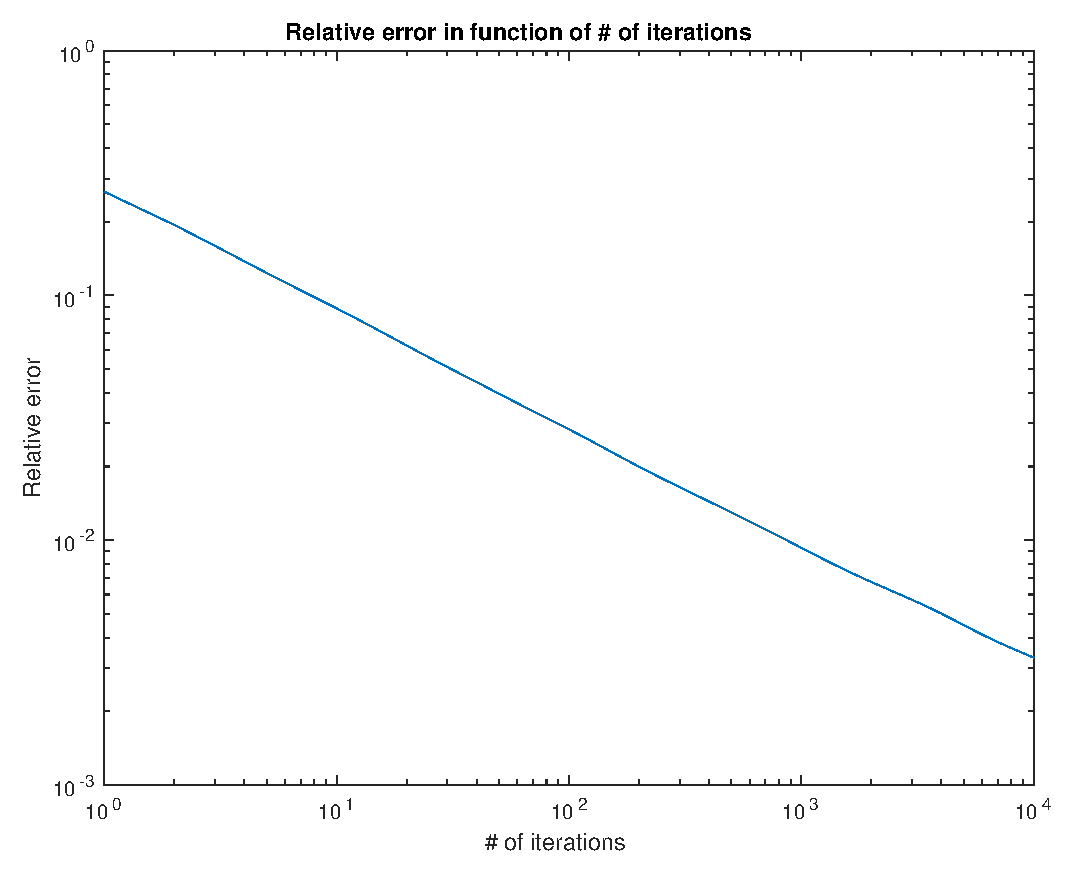
\includegraphics[scale=0.55]{opdracht4}
\caption{Opdracht 4}
\end{figure}

\lstinputlisting[language=Matlab, caption=Opdracht 4, firstline=6, lastline=13]{../opdrachten.m}



\section*{Opdracht 5}
De kleinste rang waarvoor de benaderingsfout kleiner is als $10^{-13}$ is 26.
Dit valt af te lezen van de figuur alsook in de vector \texttt{Error} in onderstaande code waarbij het 26ste element 0.000000000000003 is, terwijl het 25ste nog 0.000000000005736 is en dus groter als $10^{-13}$.
\begin{figure}[H]
\centering
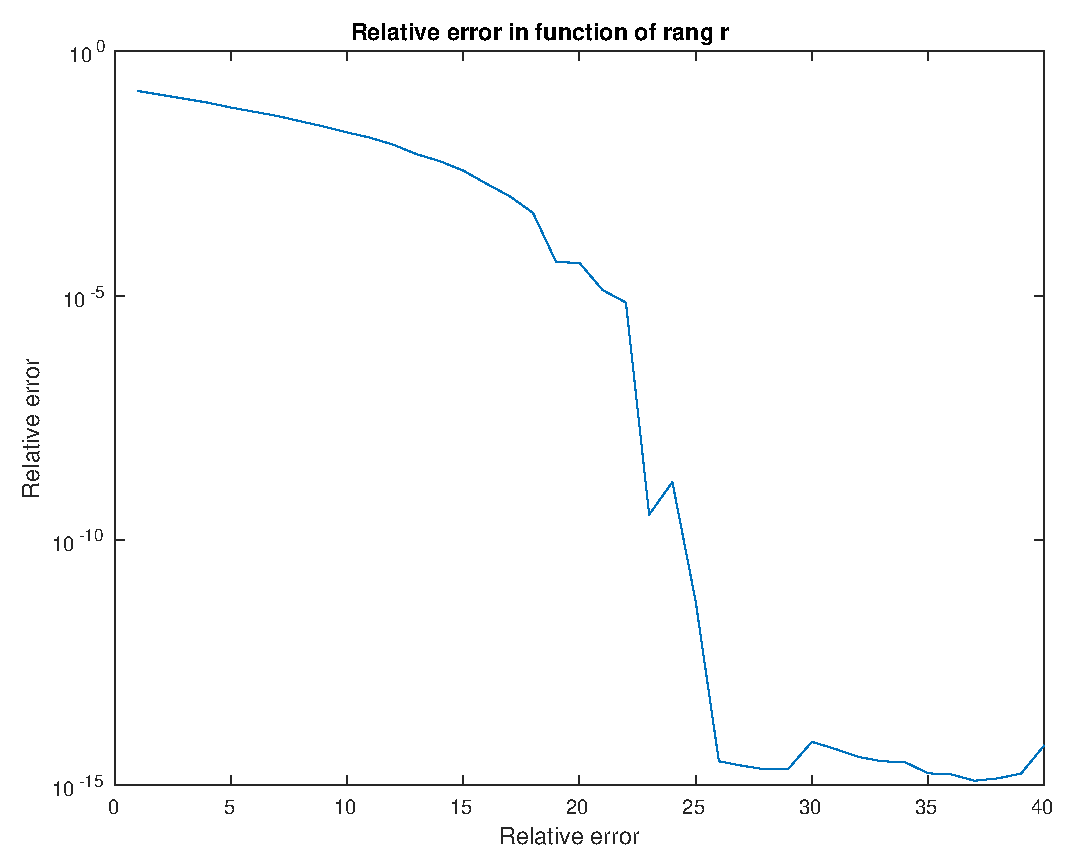
\includegraphics[scale=0.55]{opdracht5}
\caption{All approximation errors}
\end{figure}

\lstinputlisting[language=Matlab, caption=Opdracht 5]{../r0381767_plotAllApproximationErrors.m}
\lstinputlisting[language=Matlab, caption=Hulproutine voor opdracht 5]{../r0381767_predictedError.m}

\section*{Opdracht 6}

\begin{figure}[H]
\centering
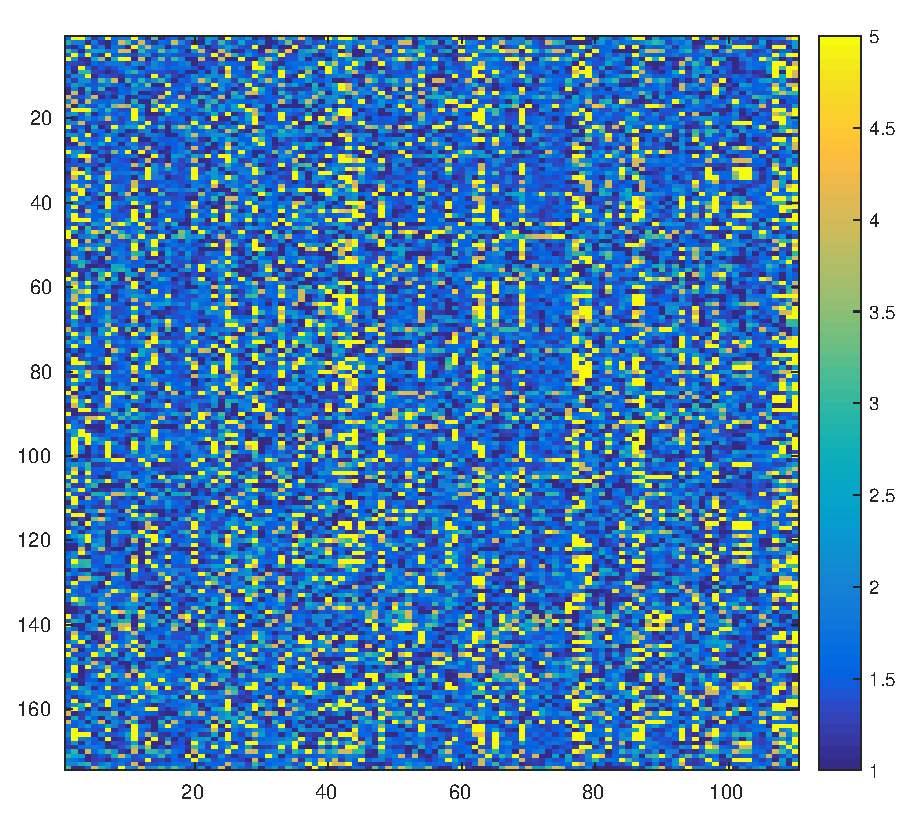
\includegraphics[scale=0.55]{opdracht6}
\caption{Predicted26}
\end{figure}

\lstinputlisting[language=Matlab, caption=Opdracht 4, firstline=19, lastline=24]{../opdrachten.m}

\section*{Opdracht 7}

\lstinputlisting[language=Matlab, caption=Opdracht 7]{../r0381767_similarBooks.m}

\section*{Opdracht 8}

\textbf{Boek 1:}
\begin{enumerate}
\item Harry Potter and the Sorcerer's Stone
\item Harry Potter and the Chamber of Secrets
\item Harry Potter And The Goblet Of Fire (Book 4)
\item Harry Potter And The Prisoner Of Azkaban
\item Harry Potter and the Order of the Phoenix (Book 5)
\item Harry Potter and the Half-Blood Prince
\end{enumerate}
\textbf{Boek 21:}
\begin{enumerate}
\item A Game of Thrones: A Song of Ice and Fire: Book One
\item A Clash of Kings: A Song of Ice and Fire: Book Two (Game of Thrones)
\item A Feast for Crows (A Song of Ice and Fire)
\end{enumerate}
\textbf{Boek 101:}
\begin{enumerate}
\item The Arrangement 2
\item The Arrangement 3 (Volume 3)
\item The Arrangement 11: The Ferro Family  (Volume 11)
\item The Arrangement 4 (Volume 4)
\item The Arrangement Vol. 8: The Ferro Family (Volume 8)
\item The Arrangement 13 (The Ferro Family) (Volume 13)
\item The Arrangement 5 (Volume 5)
\item The Arrangement 12 (The Ferro Family) (Volume 12)
\item The Arrangement 14 (The Ferro Family) (Volume 14)
\item The Arrangement 9: The Ferro Family (Volume 9)
\end{enumerate}
\end{document}